\section{紧算子的奇异分解}
\label{sec:ospec-singular}

累积积分$V$没有特征向量，从$L^2(\nu)$到另一个空间$L^2(\mu)$的积分算子更谈不上$T-\lambda I$。有限维中，矩阵的奇异值分解用输入、输出各一组标准正交方向解决这个问题，可参考\BookChapterRef{chap:singular-value-decomposition}{卷二第5章“奇异值分解”}。对紧算子，同样的构造可以通过正的紧自伴算子$T^*T$完成，而不要求原算子自伴，也不要求输入与输出位于同一空间。

本节设$H_1,H_2$是Hilbert空间，$T:H_1\to H_2$是紧算子。

\paragraph{从$T^*T$构造两组方向}
$T^*T:H_1\to H_1$是紧算子，因为它是有界算子$T^*$与紧算子$T$的复合；它自伴，并且
\[
\langle x,T^*Tx\rangle=\langle Tx,Tx\rangle=\lVert Tx\rVert^2\geq0 ,
\]
所以是正算子，特征值都非负，并且$T^*Tx=0$当且仅当$Tx=0$，即$\ker(T^*T)=\ker T$。

对$T^*T$应用定理~\ref{thm:ospec-compact-self-adjoint}，得到标准正交的特征向量$v_j$与正特征值$s_j$，按递减顺序排列。令$\sigma_j=\sqrt{s_j}$，再令$u_j=Tv_j/\sigma_j$。这组输出方向也标准正交：
\[
\langle u_j,u_k\rangle=\frac{\langle Tv_j,Tv_k\rangle}{\sigma_j\sigma_k}=\frac{\langle v_j,T^*Tv_k\rangle}{\sigma_j\sigma_k}=\frac{\sigma_k^2\langle v_j,v_k\rangle}{\sigma_j\sigma_k}=\delta_{j,k} .
\]
此外$T^*u_j=T^*Tv_j/\sigma_j=\sigma_jv_j$，所以$T$把$v_j$送到$\sigma_ju_j$，$T^*$把$u_j$送回$\sigma_jv_j$。

\begin{theorem}[紧算子的奇异分解]
\label{thm:ospec-svd}
设$T:H_1\to H_2$是紧算子，$\sigma_1\geq\sigma_2\geq\cdots>0$及标准正交序列$(v_j)\subseteq H_1$、$(u_j)\subseteq H_2$如上构造。则对每个$x\in H_1$、$y\in H_2$，
\begin{equation}
Tx=\sum_j\sigma_j\langle v_j,x\rangle u_j,\qquad T^*y=\sum_j\sigma_j\langle u_j,y\rangle v_j ,
\label{eq:ospec-svd}
\end{equation}
级数按范数收敛。$(v_j)$的闭张成为$(\ker T)^\perp$，$(u_j)$的闭张成为$\overline{\operatorname{Ran}T}=(\ker T^*)^\perp$。序列无限时$\sigma_j\to0$。
\end{theorem}

\begin{proof}
由定理~\ref{thm:ospec-compact-self-adjoint}，$(v_j)$的闭张成为$(\ker T^*T)^\perp=(\ker T)^\perp$，任意$x$可写成$x=x_0+\sum_j\langle v_j,x\rangle v_j$，$x_0\in\ker T$。把$T$作用于部分和并取极限，得$Tx=\sum_j\langle v_j,x\rangle Tv_j=\sum_j\sigma_j\langle v_j,x\rangle u_j$。

由这一展开，每个$Tx$都落在$(u_j)$的闭张成中；反之每个$u_j=T(v_j/\sigma_j)$属于$\operatorname{Ran}T$。所以$(u_j)$的闭张成等于$\overline{\operatorname{Ran}T}$，再由第~\ref{chap:linear-operators}章的正交关系，它等于$(\ker T^*)^\perp$。

关于$T^*$的展开，对任意$x$有
\[
\langle x,T^*y\rangle=\langle Tx,y\rangle=\sum_j\sigma_j\overline{\langle v_j,x\rangle}\langle u_j,y\rangle=\Bigl\langle x,\sum_j\sigma_j\langle u_j,y\rangle v_j\Bigr\rangle ,
\]
右端级数因系数平方可和而收敛，两边对一切$x$相等，故展开成立。$\sigma_j\to0$来自$s_j\to0$。
\end{proof}

数$\sigma_j$称为$T$的\term{奇异值}（singular value），$v_j$与$u_j$分别称为\term{右奇异向量}（right singular vector）与\term{左奇异向量}（left singular vector），三者合称$T$的\term{奇异系统}（singular system）。函数空间中，左右奇异向量也称左右奇异函数。

展开式\eqref{eq:ospec-svd}把$T$的作用拆成三步：读出输入在$v_j$方向上的系数，乘以$\sigma_j$，再放到输出方向$u_j$上。输入空间分成$\ker T$与$\overline{\operatorname{span}}\{v_j\}$，前者的分量在输出中完全看不见；输出空间分成$\ker T^*$与$\overline{\operatorname{span}}\{u_j\}$，前者是任何输入都到达不了的方向。两组方向一般位于不同的空间；即使$H_1=H_2$，$u_j$也未必等于$v_j$。对正的紧自伴算子，两组方向可以取得相同，奇异值就是特征值；对一般自伴算子，奇异值是特征值的绝对值，负特征值的方向上$u_j=-v_j$。

\begin{example}[累积积分的奇异分解]
\label{ex:ospec-volterra-svd}
在$L^2(0,1)$上，$(Vf)(x)=\int_0^xf(t)\,\mathrm dt$是紧算子，伴随为$(V^*g)(t)=\int_t^1g(x)\,\mathrm dx$（第~\ref{chap:linear-operators}章），于是
\[
(V^*Vf)(t)=\int_t^1\Bigl(\int_0^xf(s)\,\mathrm ds\Bigr)\mathrm dx .
\]

设$V^*Vf=sf$，$s>0$。右端是连续函数，所以$f=s^{-1}V^*Vf$连续；于是$Vf$连续可导，$V^*Vf$二次连续可导，$f$也二次连续可导。对$t$求导两次得$(V^*Vf)^\prime=-Vf$、$(V^*Vf)^{\prime\prime}=-f$，因此$sf^{\prime\prime}=-f$；又由表达式直接读出$(V^*Vf)^\prime(0)=0$、$(V^*Vf)(1)=0$，故$f^\prime(0)=0$、$f(1)=0$。满足这些条件的非零解为$f(t)=c\cos(\omega t)$，其中$\omega=s^{-1/2}$且$\cos\omega=0$，即$\omega_k=(k-\tfrac12)\pi$，$k=1,2,\ldots$。

上一节已证明$V$是单射，所以$\ker V^*V=\ker V=\{0\}$，$V^*V$的特征向量张满整个$L^2(0,1)$。由此
\begin{equation*}
\begin{gathered}
\sigma_k=\frac{1}{(k-\frac12)\pi}=\frac{2}{(2k-1)\pi},\\
v_k(t)=\sqrt2\cos\bigl((k-\tfrac12)\pi t\bigr),\qquad u_k(x)=\sqrt2\sin\bigl((k-\tfrac12)\pi x\bigr),
\end{gathered}
\end{equation*}
其中$u_k=Vv_k/\sigma_k$可直接积分验证，归一化由$\int_0^12\cos^2(\omega_kt)\,\mathrm dt=1+\sin(2\omega_k)/(2\omega_k)=1$核对。前几个奇异值约为$0.637$、$0.212$、$0.127$、$0.091$，按$1/k$的速度衰减。
\end{example}

$V$没有特征向量，却有完整的奇异系统：输入方向是余弦族，输出方向是正弦族，两组方向不同。这说明奇异分解确实不依赖自伴性，它对每个紧算子都存在。

\paragraph{截断奇异分解}
只保留前$m$项，得到秩不超过$m$的算子
\[
T_mx=\sum_{j\leq m}\sigma_j\langle v_j,x\rangle u_j .
\]
下面的定理说明，截断误差恰为第一个被舍弃的奇异值，并且没有任何秩不超过$m$的算子能做得更好。正奇异值只有有限个时，约定用尽之后的$\sigma_j=0$。

\begin{theorem}[截断奇异分解的误差]
\label{thm:ospec-svd-truncation}
在定理~\ref{thm:ospec-svd}的条件下，$\lVert T-T_m\rVert=\sigma_{m+1}$；并且对每个秩不超过$m$的有界算子$F:H_1\to H_2$，都有$\lVert T-F\rVert\geq\sigma_{m+1}$。
\end{theorem}

\begin{proof}
第一步，计算截断误差。由式\eqref{eq:ospec-svd}及$(u_j)$的正交性，
\[
\lVert(T-T_m)x\rVert^2=\sum_{j>m}\sigma_j^2\lvert\langle v_j,x\rangle\rvert^2\leq\sigma_{m+1}^2\sum_{j>m}\lvert\langle v_j,x\rangle\rvert^2\leq\sigma_{m+1}^2\lVert x\rVert^2 ,
\]
最后一步是Bessel不等式。若$\sigma_{m+1}>0$，取$x=v_{m+1}$时等号成立，所以$\lVert T-T_m\rVert=\sigma_{m+1}$。

第二步，证明下界。不妨设$\sigma_{m+1}>0$。令$W=\operatorname{span}\{v_1,\ldots,v_{m+1}\}$，它是$m+1$维的。$F$把$W$映入维数不超过$m$的$\operatorname{Ran}F$，由维数公式，存在单位向量$x\in W$使$Fx=0$。写$x=\sum_{j\leq m+1}c_jv_j$，$\sum_j\lvert c_j\rvert^2=1$，则
\[
\lVert(T-F)x\rVert^2=\lVert Tx\rVert^2=\sum_{j\leq m+1}\sigma_j^2\lvert c_j\rvert^2\geq\sigma_{m+1}^2 .
\]
因此$\lVert T-F\rVert\geq\sigma_{m+1}$。
\end{proof}

图~\ref{fig:ospec-svd-decay}在累积积分上展示这一结论。保留前三项时误差为$\sigma_4\approx0.091$；奇异值衰减越快，同样秩的截断误差越小。奇异值越小的方向振荡越快：$V$是积分，它把快速振荡的输入平均掉，输出的幅度只剩$1/\omega_k$倍。对比$\ell^2$上的$A(x_n)=(x_n/n)$，它是正自伴算子，奇异值就是特征值$1/n$，左右奇异向量都是$e_n$，第~\ref{chap:linear-operators}章对它的坐标截断正是截断奇异分解。

\begin{figure}[!htb]
  \centering
  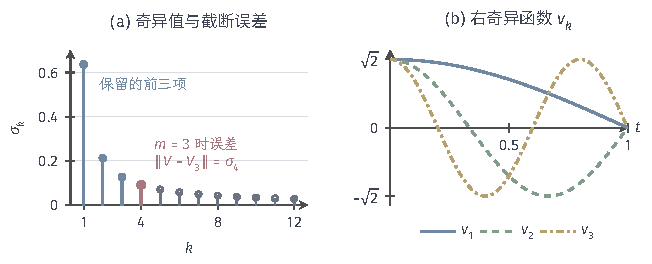
\includegraphics[width=110.3mm]{figures/02-abstract-mathematics/03-function-spaces/tikz/c3-svd-decay/figure.pdf}
  \caption{累积积分$(Vf)(x)=\int_0^xf$在$L^2(0,1)$上的奇异分解。(a)~奇异值$\sigma_k=2/((2k-1)\pi)$；保留前三项（蓝色）时，算子范数误差等于第四个奇异值$\sigma_4\approx0.091$（红色），后面的奇异值（空心）全部被舍去；(b)~前三个右奇异函数$v_k(t)=\sqrt2\cos((k-\frac12)\pi t)$，序号越大振荡越快。}
  \label{fig:ospec-svd-decay}
\end{figure}

小奇异值对正向逼近是好消息：舍去它们，误差很小。对反向求解却是坏消息：从输出恢复输入，要把这些方向上的系数除以$\sigma_j$。这一障碍是第~\ref{chap:linear-operator-equations}章讨论第一类方程时的核心问题。
